\documentclass{article}
\usepackage{graphicx} 
\usepackage{hyperref}
\title{COP701 Sample Test cases}
\date{August 2024}
\begin{document}

\section{Introduction to IIT Delhi}
\subsection{Overview}
\subsubsection{History}

\textit{Indian Institute of Technology Delhi (IIT Delhi) is one of the premier engineering institutes in India.}
\textbf{Founded in 1961, IIT Delhi has grown into a world-class institution known for its cutting-edge research and academic excellence.}

\hrule

\textbf{IIT Delhi} is located in Hauz Khas, New Delhi. It offers \textbf{undergraduate, postgraduate, and doctoral program} in various fields of \textit{engineering and technology}.\par
The institute is renowned for its rigorous academic programs and distinguished faculty.

\href{https://www.iitd.ac.in}{IIT Delhi Official Website}

\begin{itemize}
    \item Established: 1961
    \item Location: Hauz Khas, New Delhi
    \item Programs: B.Tech, M.Tech, Ph.D., and more
\end{itemize}

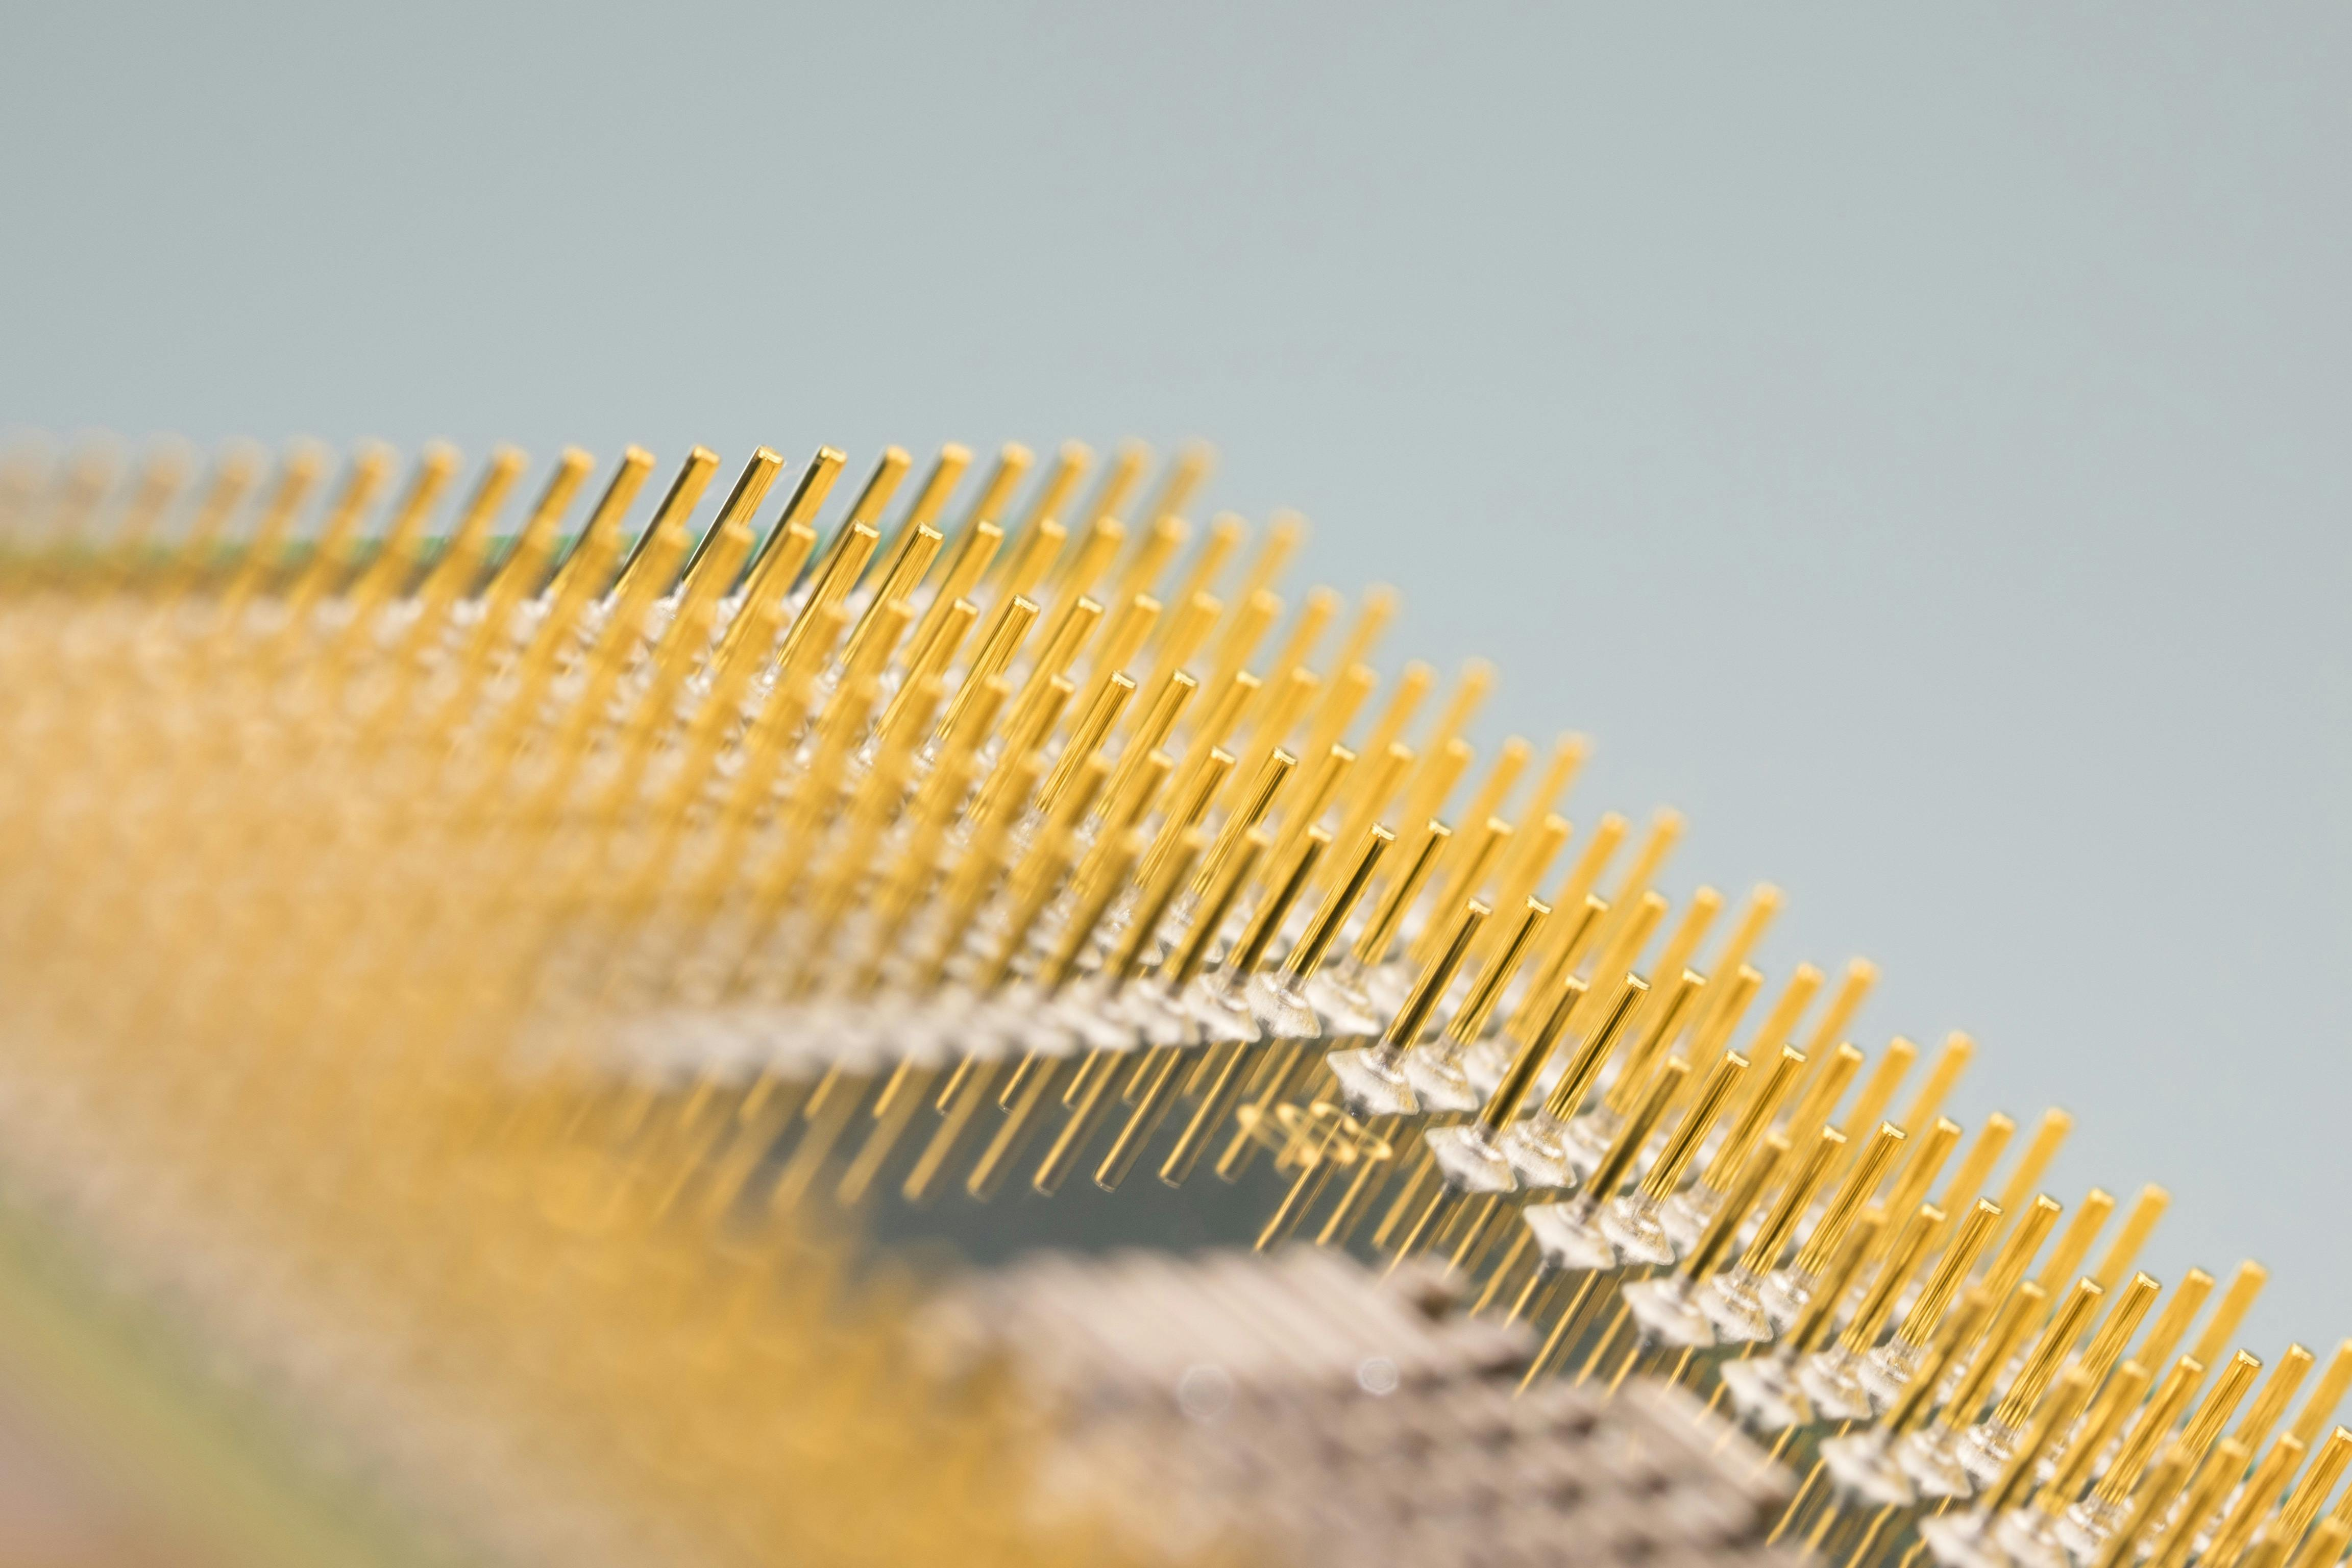
\includegraphics[width=0.5\textwidth]{images/technology.jpg}

\begin{enumerate}
    \item Campus Facilities
    \item Research Opportunities
    \item Alumni Achievements
\end{enumerate}


    
\end{document}
